\section{Results}
\label{sec:results}
\subsection{Discrimination and the matched model hierarchy}
All 30 principal runs completed training and formal evaluation; the supplementary mean-pooling model contributed ten further completed runs. Forty evaluation receipts and their 120 registered report identities were verified. All holdout evaluations used the same 175 patients and 56 positive labels. Unless stated otherwise, each reported number first averages five fold metrics within a seed, then equally averages seeds 21 and 44. We present one combined estimate per model and landmark.
\begin{table*}[t]
\centering
\small
\caption{Performance on the fixed internal holdout (175 patients, 56 pCR positive). Each value averages five fold metrics within a seed, then equally averages seeds 21 and 44. Macro averages the three landmarks. AP denotes average precision; F1 uses threshold 0.5.}
\label{tab:main}
\begin{tabular}{llrrr}
\toprule
Model & Landmark & AUROC & AP & F1 \\
\midrule
NoJEPA & T0 & 0.7151 & 0.5752 & 0.5334 \\
NoJEPA & T1 & 0.7166 & 0.5815 & 0.5347 \\
NoJEPA & T2 & 0.7154 & 0.5751 & 0.5316 \\
NoJEPA & Macro & 0.7157 & 0.5773 & 0.5333 \\
DirectReadout & T0 & 0.7264 & 0.5863 & 0.5343 \\
DirectReadout & T1 & 0.7285 & 0.5911 & 0.5369 \\
DirectReadout & T2 & 0.7281 & 0.5937 & 0.5562 \\
DirectReadout & Macro & 0.7277 & 0.5904 & 0.5425 \\
ForecastAttention & T0 & 0.7323 & 0.5933 & 0.5391 \\
ForecastAttention & T1 & 0.7363 & 0.5976 & 0.5524 \\
ForecastAttention & T2 & 0.7393 & 0.5998 & 0.5556 \\
ForecastAttention & Macro & 0.7360 & 0.5969 & 0.5490 \\
\bottomrule
\end{tabular}
\end{table*}


\fullmodel{} achieved AUROCs of 0.7323, 0.7363, and 0.7393 at T0, T1, and T2, with AP values of 0.5933, 0.5976, and 0.5998 (Fig.~\ref{fig:discrimination}). Its landmark-macro AUROC/AP/F1 was 0.7360/0.5969/0.5490, compared with 0.7157/0.5773/0.5333 for \nojepa{} and 0.7277/0.5904/0.5425 for \direct{}. The complete model therefore had the highest combined macro values of these three metrics among the principal variants. At T2, however, \direct{} retained a slightly higher F1 (0.5562 versus 0.5556), demonstrating that the ranking is not uniform across metrics and landmarks.

\begin{figure*}[t]
\centering
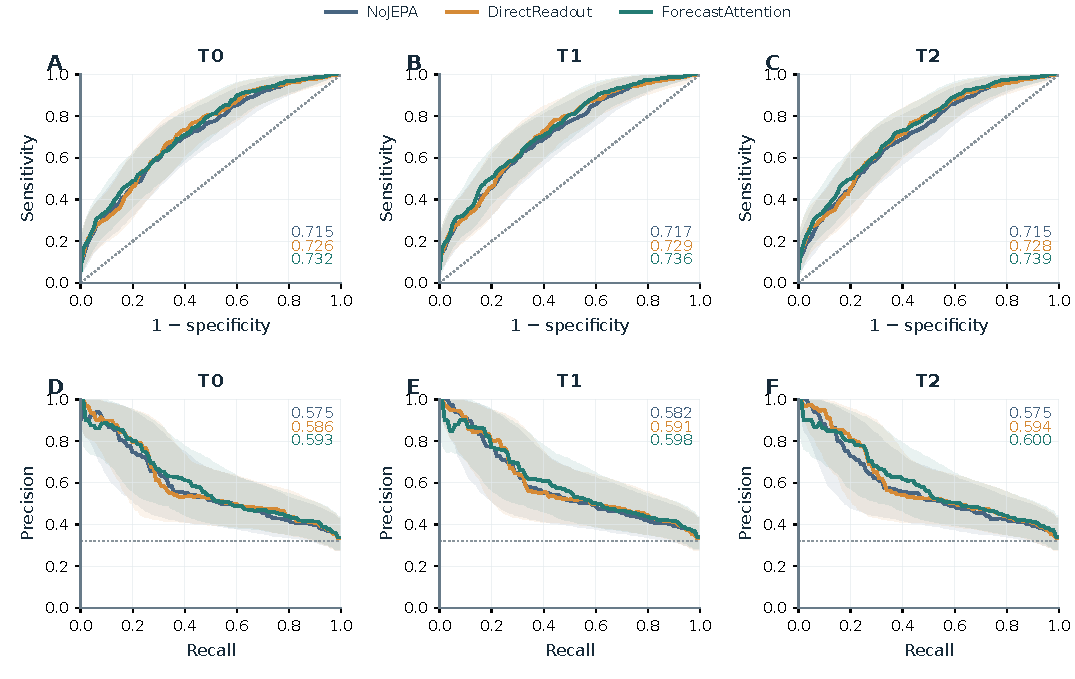
\includegraphics[width=\textwidth]{figures/discrimination.pdf}
\caption{Discrimination across matched landmarks. (A--C) ROC curves; (D--F) precision--recall curves. Curves are calculated separately in each fold model, then averaged within seed and across seeds 21/44. Shading shows pointwise 95\% paired patient-bootstrap intervals conditional on the fitted models. Colored values are the corresponding fold-then-seed mean AUROC or AP; interpolated curve areas need not equal these separately calculated statistics. The dotted PR reference is the 0.32 positive prevalence.}
\label{fig:discrimination}
\end{figure*}

Adding future-state supervision under direct readout increased macro AUROC by 0.0120, AP by 0.0131, and F1 by 0.0092. Adding the complete forecast-attention readout gave a further AUROC increase of 0.0083, AP increase of 0.0065, and F1 increase of 0.0065 relative to \direct{}. The first comparison isolates the auxiliary objective more closely; the second jointly changes the readout information, pooling, and classifier input width. Relative to \meanmodel{}, the full model increased macro AUROC/AP/F1 by 0.0032/0.0092/0.0163 (Table~\ref{tab:pooling}). These descriptive differences do not establish that attention alone causes the complete model's benefit.

Paired patient intervals clarify the strength and limits of these comparisons (Fig.~\ref{fig:paired}). The macro AUROC difference was +0.0203 [0.0042, 0.0381] for \fullmodel{} versus \nojepa{}, and +0.0120 [0.0011, 0.0242] for \direct{} versus \nojepa{}. The additional difference between \fullmodel{} and \direct{} was +0.0083 [$-0.0041$, 0.0215]. AP and F1 differences between the complete model and either direct control had intervals including zero. The intervals condition on retrospectively selected fitted models; exclusion of zero for some AUROC contrasts does not remove selection uncertainty or make this a confirmatory study.

\begin{figure*}[t]
\centering
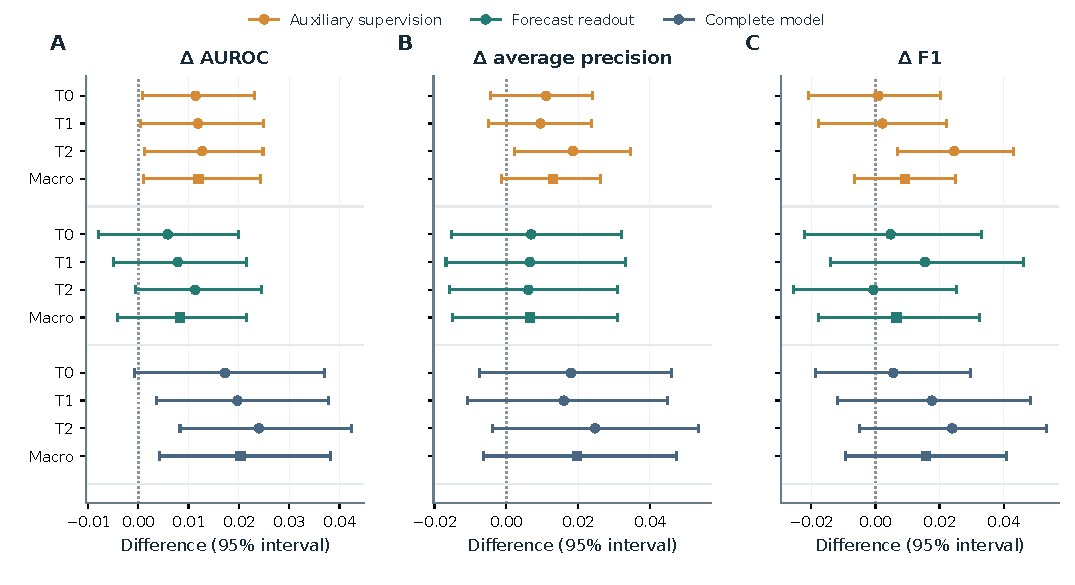
\includegraphics[width=\textwidth]{figures/paired_comparisons.pdf}
\caption{Paired model differences at T0, T1, T2, and the landmark macro. Colors distinguish the auxiliary-supervision contrast, the additional forecast-readout contrast, and the complete-model contrast. Squares denote macro estimates; bars are 95\% patient-bootstrap intervals, with identical patient draws shared across models, folds, seeds, and landmarks. Fold or seed counts are not independent patient sample sizes.}
\label{fig:paired}
\end{figure*}

\subsection{Threshold behavior and class imbalance}
\begin{table*}[t]
\centering
\small
\caption{Extended threshold-dependent metrics at probability threshold 0.5. Values first average five fold metrics within each seed and then equally average seeds 21 and 44 on the same 175 holdout patients; Macro equally averages landmarks. PPV and NPV denote positive and negative predictive value; BA is balanced accuracy.}
\label{tab:extended_operating}
\begin{tabular}{llrrrrrr}
\toprule
Model & Stage & Sens. & Spec. & PPV & NPV & BA & MCC \\
\midrule
NoJEPA & T0 & 0.593 & 0.708 & 0.493 & 0.790 & 0.651 & 0.292 \\
NoJEPA & T1 & 0.580 & 0.727 & 0.501 & 0.788 & 0.654 & 0.298 \\
NoJEPA & T2 & 0.589 & 0.710 & 0.492 & 0.788 & 0.650 & 0.290 \\
NoJEPA & Macro & 0.588 & 0.715 & 0.495 & 0.789 & 0.651 & 0.293 \\
\midrule
DirectReadout & T0 & 0.579 & 0.726 & 0.502 & 0.787 & 0.652 & 0.296 \\
DirectReadout & T1 & 0.589 & 0.716 & 0.497 & 0.788 & 0.653 & 0.295 \\
DirectReadout & T2 & 0.623 & 0.711 & 0.505 & 0.802 & 0.667 & 0.320 \\
DirectReadout & Macro & 0.597 & 0.718 & 0.501 & 0.792 & 0.657 & 0.304 \\
\midrule
ForecastAttention & T0 & 0.629 & 0.674 & 0.485 & 0.803 & 0.651 & 0.295 \\
ForecastAttention & T1 & 0.680 & 0.634 & 0.479 & 0.816 & 0.657 & 0.305 \\
ForecastAttention & T2 & 0.693 & 0.621 & 0.475 & 0.824 & 0.657 & 0.304 \\
ForecastAttention & Macro & 0.667 & 0.643 & 0.480 & 0.814 & 0.655 & 0.301 \\
\bottomrule
\end{tabular}
\end{table*}

Extended metrics reveal a trade-off hidden by AUROC and F1 alone (Table~\ref{tab:extended_operating}). At threshold 0.5, \fullmodel{} had macro sensitivity 0.6673 and NPV 0.8143, compared with 0.5970 and 0.7922 for \direct{}. The increase in sensitivity (+0.0702 [0.0399, 0.1051]) was accompanied by a specificity decrease from 0.7176 to 0.6431 ($-0.0745$ [$-0.0949$, $-0.0554$]) and a PPV decrease from 0.5011 to 0.4796. The full model was therefore more likely to identify pCR-positive patients while also assigning more non-pCR patients a positive prediction.

\direct{} had the highest macro balanced accuracy (0.6573) and MCC (0.3037), compared with 0.6552 and 0.3013 for \fullmodel{} and 0.6513 and 0.2931 for \nojepa{}. Raw macro accuracy was 0.6790, 0.6509, and 0.6743, respectively. Because predicting every patient as non-pCR gives an accuracy of 0.68, accuracy alone does not demonstrate useful discrimination in this imbalanced cohort. Balanced accuracy, class-specific rates, and threshold-free discrimination provide the necessary context.

Validation-selected Youden thresholds did not uniformly improve classification (Table~\ref{tab:extended_threshold}). For \fullmodel{}, sensitivity fell to 0.6405 and specificity increased to 0.6605; macro F1 fell from 0.5490 to 0.5418. The corresponding F1 values changed from 0.5333 to 0.5349 for \nojepa{} and from 0.5425 to 0.5371 for \direct{}. Thus a different validation objective changes the operating point without guaranteeing a higher holdout F1. No holdout labels were used to select these thresholds.

\subsection{Longitudinal information and probability quality}
The same-patient T2--T0 AUROC change was +0.0071 [0.0006, 0.0138] for \fullmodel{}, +0.0003 [$-0.0059$, 0.0067] for \nojepa{}, and +0.0016 [$-0.0038$, 0.0064] for \direct{}. The full model's sensitivity increased from 0.6286 to 0.6929, while specificity decreased from 0.6740 to 0.6210. This illustrates why a positive longitudinal AUROC trend should be considered alongside threshold-dependent errors. Outcome-conditioned score-change distributions are provided in Fig.~\ref{fig:scorechanges}; they average within-model histograms and do not turn the fitted models into a probability ensemble.

\begin{table*}[t]
\centering
\small
\caption{Probability quality averaged across landmarks after fold and seed aggregation. Lower is better. ECE uses ten equal-width bins.}
\label{tab:calibration}
\begin{tabular}{lrrr}
\toprule
Model & NLL & Brier & ECE \\
\midrule
NoJEPA & 0.6018 & 0.2083 & 0.1323 \\
DirectReadout & 0.5959 & 0.2049 & 0.1280 \\
ForecastAttention & 0.6102 & 0.2118 & 0.1544 \\
\bottomrule
\end{tabular}
\end{table*}

The complete model's higher discrimination did not imply better probabilities. Its macro NLL/Brier/ECE was 0.6102/0.2118/0.1544, compared with 0.5959/0.2049/0.1280 for \direct{} and 0.6018/0.2083/0.1323 for \nojepa{}. Reliability curves in Fig.~\ref{fig:calutility} show how observed response frequency relates to predicted probability. The Brier score and ECE of \fullmodel{} worsened toward T2 even as AUROC increased (Fig.~\ref{fig:longitudinal}), reinforcing the distinction between ranking and calibrated probability estimation. Point estimates and conditional patient-bootstrap intervals for all 14 macro metrics are collected in Table~\ref{tab:extended_macro}.

\begin{figure*}[t]
\centering
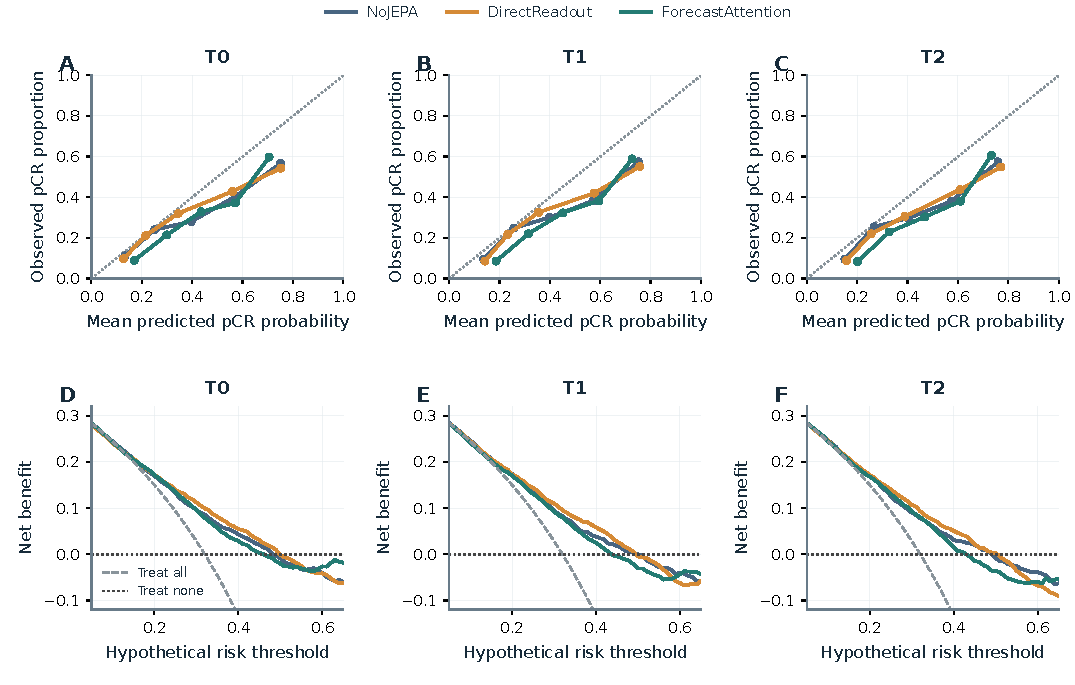
\includegraphics[width=\textwidth]{figures/calibration_utility.pdf}
\caption{Probability quality and hypothetical decision utility. (A--C) Reliability diagrams use five equal-count probability-rank groups within each fitted model (35 patients per group); group coordinates are then averaged over folds and seeds. These groups describe calibration and differ from the ten fixed probability bins used for ECE. (D--F) Net-benefit curves under generic threshold-based positive actions, with treat-all and treat-none references. All curves use the original probabilities, without recalibration. No particular escalation or de-escalation decision is validated by this analysis.}
\label{fig:calutility}
\end{figure*}

\subsection{Hypothetical net benefit}
Decision curves did not preserve the discrimination ranking across thresholds. At a hypothetical risk threshold of 0.30, macro net benefit was 0.1097 for \direct{} and 0.0943 for \fullmodel{}, although the latter had higher AUROC and AP. At threshold 0.50, all three principal models had non-positive macro net benefit relative to the zero reference. These values depend on the mathematical threshold trade-off, pCR prevalence, and the uncalibrated model outputs. They indicate that a ranking advantage alone does not establish a preferable clinical action rule.

\subsection{Exploratory biological and acquisition-related subgroups}
Figure~\ref{fig:subgroups} and Table~\ref{tab:subgroups} show heterogeneity in the combined results. The HR-positive/HER2-negative group contained 68 patients but only 11 pCR-positive cases. Its macro AUROC difference for \fullmodel{} versus \nojepa{} was +0.0522 [0.0095, 0.0995]. In contrast, the HR-positive/HER2-positive group (31 patients, 12 positive) had a difference of $-0.0154$ [$-0.0780$, 0.0473]. The HR-negative/HER2-positive group contained only 14 patients and had a wide interval, while the HR-negative/HER2-negative group had a +0.0219 difference with an interval including zero. These unadjusted subgroup summaries are exploratory, and differences in whether an interval includes zero are not evidence of a subgroup interaction.

The threshold trade-off was also group dependent. In HR-positive/HER2-negative patients, the full model's sensitivity/specificity was 0.2030/0.9170, compared with 0.0970/0.9690 for \nojepa{}. Improved ranking therefore coexisted with low sensitivity at 0.5 in that group. Age-based and source-namespace summaries are descriptive; the two source namespaces belong to the same clinical release and do not form an external validation. Only 11 holdout patients had partial clipping of the largest predicted baseline component, including one positive outcome. AUROC and AP were therefore suppressed for that group under the minimum-outcome rule, rather than interpreting an unstable estimate.

\begin{figure*}[t]
\centering
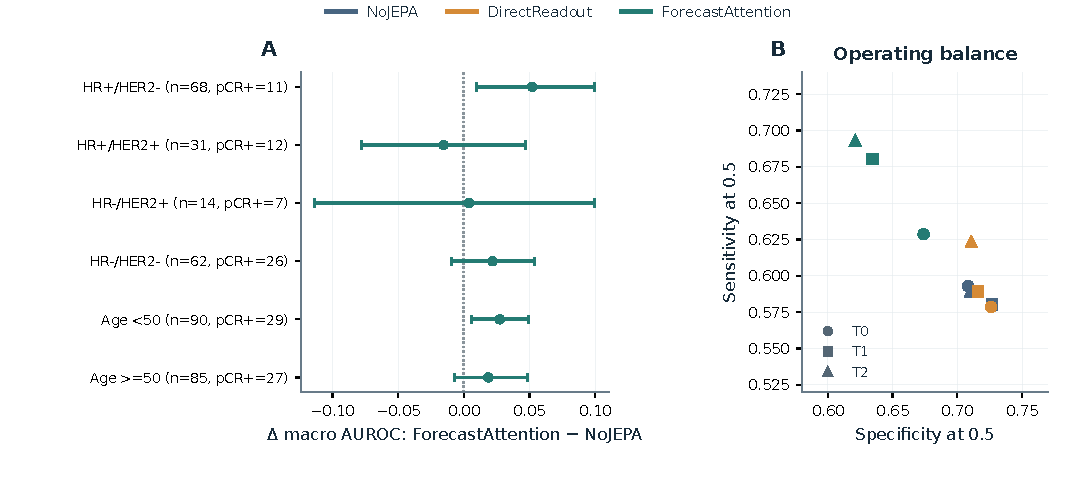
\includegraphics[width=\textwidth]{figures/subgroup_operating.pdf}
\caption{Exploratory heterogeneity and operating-point behavior. (A) Macro AUROC differences between ForecastAttention and NoJEPA within HR/HER2 and age groups, with patient counts, positive-outcome counts, and unadjusted paired intervals. No subgroup-interaction claim is made. (B) Specificity and sensitivity at threshold 0.5, showing the operating-point movement across landmarks. Colors identify models and markers identify landmarks.}
\label{fig:subgroups}
\end{figure*}

\subsection{Archived forecast and gradient diagnostics}
The existing fixed-training-probe archive provides limited mechanistic evidence, distinct from the holdout pCR evaluation (Fig.~\ref{fig:mechanism}). At the illustrative common epoch 20, \direct{} achieved copy-normalized forecast skill of +0.0227, +0.0368, and +0.1584 for one-, two-, and three-step horizons. The corresponding values for \fullmodel{} were $-0.0295$, $-0.0271$, and +0.0174 (Table~\ref{tab:worldprobe}). Consequently, the better pCR ranking of the complete model cannot simply be explained as more accurate latent forecasting under this diagnostic. This diagnostic admits a forecast target only when the landmark, target, and every intervening canonical visit are actually observed; missing intermediate visits exclude that chain. Its eligible population therefore differs by horizon and is narrower than the missing-target-masked training objective. Long-horizon eligibility was only 5--9 patients per training probe, and these measurements are not best-checkpoint holdout forecast accuracy.

The archived task-loss gradient norm in the predictor was zero for \direct{} and averaged 0.8205 for \fullmodel{} at epoch 20; the weighted rollout-gradient norms were 0.1364 and 0.1743, respectively. This supports the expected difference in gradient routing: the full classifier can shape the forecast predictor, while the direct classifier does not read its predicted states. Gradient magnitude itself is not an effect size or evidence that the forecast captures more accurate tumor biology. \nojepa{} has no available world-performance diagnostic and is not assigned an artificial zero error or zero skill.

\begin{figure*}[t]
\centering
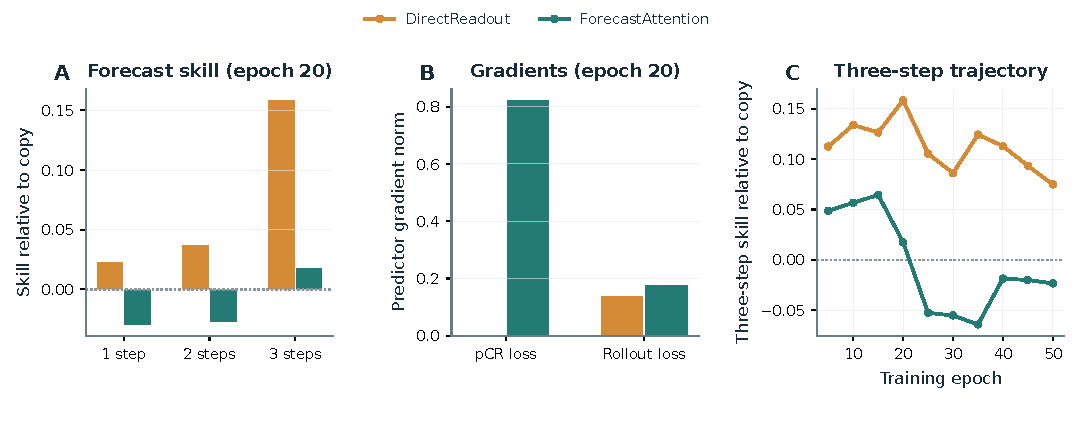
\includegraphics[width=\textwidth]{figures/forecast_mechanism.pdf}
\caption{Archived fixed-training-probe diagnostics. (A) Copy-normalized latent forecast skill at common epoch 20; positive values outperform holding the current state constant in the same snapshot's EMA coordinates. (B) Predictor gradient norms from pCR and weighted rollout losses. (C) Three-step skill over common archived training epochs. Values average folds within seed and then seeds 21/44. Forecast targets require the real landmark, target, and all intermediate visits, so eligibility varies by horizon. These are training diagnostics, not holdout or best-checkpoint mechanism evaluations; three-step eligibility is only 5--9 patients per probe.}
\label{fig:mechanism}
\end{figure*}
